% Use actual IEEE Times-compatible bold/italic fonts.
\RequirePackage[T1]{fontenc}
\documentclass[conference]{IEEEtran}
\usepackage{cite}
\usepackage{graphicx}
\usepackage{array}
\usepackage{amsmath,amssymb,amsfonts}
\usepackage{textcomp}
\usepackage[hyphens]{url}
\usepackage[hidelinks]{hyperref}
\usepackage{xcolor}
\emergencystretch=3em
\setcounter{dbltopnumber}{2}
\renewcommand{\dbltopfraction}{0.95}
\renewcommand{\dblfloatpagefraction}{0.85}
\renewcommand{\textfraction}{0.05}
\newcommand{\CADDAM}{CADD\allowbreak{}+\allowbreak{}AlphaMissense}
\newcommand{\GCNCADDAM}{GCN\allowbreak{}+\allowbreak{}CADD\allowbreak{}+\allowbreak{}AlphaMissense}

\title{Auditing PPI Graph Augmentation for Missense Variant Pathogenicity Prediction under Topology, Connectivity and Homology Constraints}

\author{\IEEEauthorblockN{Yuxin Tian, Xianguo Zhang\textsuperscript{*}, Weibo Meng, Jieqi Yin, and Yongqin Jin}
\IEEEauthorblockA{College of Computer Science (College of Software), College of Artificial Intelligence\\
Inner Mongolia University, Hohhot 010021, China\\
Email: yuxin\_t02@163.com; 2595083628@qq.com\\
\textsuperscript{*}Corresponding author: Xianguo Zhang}}
\hypersetup{pdfauthor={Yuxin Tian, Xianguo Zhang, Weibo Meng, Jieqi Yin, Yongqin Jin}}

\begin{document}
\maketitle


\begin{abstract}
\bfseries\boldmath
Protein-protein interaction (PPI) graphs provide molecular context for missense variant pathogenicity prediction. We audit fixed two-hop PPI-GCN propagation of protein language model embeddings on 177,213 ClinVar variants, separating connectivity, topology, homology and complementarity to CADD and AlphaMissense. Only the downstream classifier is trained. Three-seed mean AUC increased from 0.7835 to 0.7950, but the protein-clustered 95\% interval for the ensemble AUC gain included zero. Graph fusion added a small benefit over raw-embedding fusion under the original split; its added value over strong scores remained uncertain under homology-aware splitting. Exploratory topology and prediction-transition analyses identified candidate contexts for these effects. On 10,785 external UniProt variants, STRING propagation improved mean AUC from 0.6932 to 0.7304; the protein-bootstrap 95\% interval for the ensemble AUC gain excluded zero. A BioGRID comparison showed uncertain external gains over raw embeddings. PPI context therefore provides network- and split-dependent information rather than a uniform benefit. These transductive fixed-propagation results should not be generalized to trained graph neural networks.

\end{abstract}

\begin{IEEEkeywords}
\bfseries\boldmath
Missense variant pathogenicity, protein-protein interaction networks, graph augmentation, protein language models, homology-aware evaluation.
\end{IEEEkeywords}

\section{Introduction}

Missense variant pathogenicity prediction has been advanced by established methods such as CADD, REVEL, MVP, PrimateAI, EVE and AlphaMissense \cite{Kircher2014CADD,Ioannidis2016REVEL,Qi2021MVP,Sundaram2018PrimateAI,Frazer2021EVE,Cheng2023AlphaMissense}, as well as by protein language models such as ESM \cite{Lin2023ESM}. These approaches capture sequence, evolutionary and annotation-derived signals. Disease-associated proteins are also embedded in molecular interaction networks, and disease-associated mutations can perturb protein-protein and other macromolecular interactions \cite{Barabasi2011NetworkMedicine,Menche2015DiseaseModules,Sahni2015InteractionPerturbation,Chen2018InteractomePerturbation}. PPI graphs provide an additional source of context for missense variant prediction.

Earlier approaches incorporated protein-interaction and other molecular-network features into single-amino-acid variant prioritization, showing that network context can provide information complementary to sequence, structure and annotation features \cite{Yates2014SuSPect,Ozturk2022NetworkFeatures}. More recent graph-based variant predictors include graph attention models for missense effects, heterogeneous gene-variant graph approaches, multimodal variant graph methods and disease-specific graph models \cite{Zhang2022gMVP,Cheng2021VEGN,Yu2025GNNMAP,Ghadie2025DiseaseSpecificGNN}. These studies establish the relevance of relational structure to variant interpretation. We focus on how to interpret gains obtained by propagating protein language model embeddings over a shared STRING PPI graph before variant-level classification.

A shared-graph setting mixes several effects. Train, validation and test variants may have distinct protein identifiers while their proteins remain directly connected in the same PPI graph. Related proteins may also cross partitions when homology is not explicitly controlled \cite{Littmann2022ProteinMLTips,Teufel2023GraphPart}. Strong variant-effect predictors such as CADD and AlphaMissense can further reduce the marginal contribution of graph propagation. We evaluate protein-topology correspondence, graph connectivity, protein-level uncertainty, homology-aware performance and complementarity to established predictors.

We conduct a systematic audit using a reconstructed ClinVar-STRING missense dataset and evaluate raw ESM representations, fixed PPI-GCN propagation, CADD, AlphaMissense and fusion models. The study separates connectivity and representation complementarity, tests strong-predictor fusion under homology-aware splitting, and examines exploratory topology contexts and error transitions. External-source and second-network validation test the transfer and network dependence of the findings.

\section{Materials and Methods}

\subsection{Dataset and graph construction}

ClinVar variant annotations were obtained from the official NCBI ClinVar FTP tab-delimited variant-summary file \cite{Landrum2020ClinVar}. We used frozen processed ClinVar tables identified by checksums; the exact historical content-release date could not be verified. We reconstructed a filtered, non-conflicting missense dataset and mapped variants to STRING human protein identifiers. We retained GRCh38 germline missense SNVs with criteria-supported review status, combined pathogenic and likely pathogenic records into the positive class, combined benign and likely benign records into the negative class, removed uncertain or conflicting records, and collapsed duplicate VariationIDs. The final ClinVar-STRING dataset contained 177,213 missense variants mapped to 14,123 labelled STRING proteins. The propagation graph contained 19,622 STRING protein nodes and 13,715,404 directed edge-index entries from the STRING v12 protein-association network \cite{Szklarczyk2023STRING}. We used this network as PPI context; its association evidence extends beyond direct physical interactions.

\subsection{Protein representations and PPI propagation}

Raw protein features were generated using the ESM-2 650M checkpoint, with 1,280-dimensional protein-level vectors obtained by residue averaging \cite{Lin2023ESM}. PPI-GCN embeddings were computed by fixed two-hop GCN-style propagation over the normalized STRING graph \cite{Kipf2017GCN}. We use ``PPI-GCN'' as shorthand for fixed GCN-style propagation of ESM features; no graph-convolution parameters were learned. Fixed propagation isolates topology-induced smoothing from capacity gains due to trainable graph layers and provides a controlled representation for the audit. Let $X$ denote the raw ESM protein-representation matrix. The full-graph implementation added self-loops before symmetrization and summed duplicate contributions: $\tilde{A}=(E+I)+(E+I)^{\mathrm{T}}$, where $E$ is the edge-index count matrix and $\tilde{D}$ is the weighted degree matrix of $\tilde{A}$. STRING confidence scores were not propagation weights. We computed the symmetrically normalized adjacency matrix as
\begin{equation}
\hat{A}=\tilde{D}^{-\frac{1}{2}}\tilde{A}\tilde{D}^{-\frac{1}{2}},
\end{equation}
\begin{equation}
H=\frac{1}{3}\left(X+\hat{A}X+\hat{A}^{2}X\right).
\end{equation}
The fixed two-hop PPI-GCN representation $H$ averages the original ESM features, one-hop PPI-smoothed features and two-hop PPI-smoothed features. Propagation used only graph structure and ESM features; downstream classification used the representation of each variant's mapped STRING protein. The full graph contained train, validation and test nodes with their ESM features, making the evaluation transductive. A representation-only model assigns one protein-context score to all variants of a protein and cannot resolve within-protein residue effects.

\subsection{Splits, classifiers and external predictors}

The original split assigned train, validation and test variants by STRING protein ID, with no shared proteins across partitions. The split contained 141,864 training variants, 17,129 validation variants and 18,220 test variants. The homology-aware split used MMseqs-derived protein clusters with minimum identity 0.40 and coverage 0.50 (mode 0); each cluster was assigned wholly to one partition, preserving the same row counts \cite{Steinegger2017MMseqs2}. We use this split as a stress test. Its test positive rate was 10.56\%, compared with 31.95\% in the original split, which limits direct cross-split AUPRC comparison.

All representation and fusion models used downstream MLP classifiers selected by validation AUC and optimized with Adam \cite{Kingma2015Adam}. Multi-feature models used 512/128 hidden units and dropout 0.3; historical single-score baselines used 32/16 units and dropout 0.2. Architecture-matched comparisons used the same 512/128 hidden-layer architecture and preprocessing, although score-only models had fewer input-layer parameters. Current matched runs used seeds 42--44, batch size 1,024, learning rate $10^{-3}$, weight decay $10^{-5}$, at most 50 epochs and patience five. Historical negative controls had different seeds, budgets and self-loop conventions (Table~\ref{tab:run_sources}; Supplementary Table 8); current controls use the full-graph operator throughout. Training used class-weighted binary cross-entropy with positive-class weight $N_{\mathrm{negative}}/N_{\mathrm{positive}}$. CADD v1.7 and AlphaMissense scores \cite{Kircher2014CADD,Schubach2024CADDv17,Cheng2023AlphaMissense} covered 99.995\% and 96.92\% of variants. Missing scores were imputed with training-set medians, with an AlphaMissense missingness indicator. Inputs were not standardized; alternative feature scaling was not evaluated.

\subsection{Audit analyses}

Uncertainty was assessed using variant-level bootstrap and protein-clustered bootstrap \cite{Efron1993Bootstrap}. Connectivity tests removed direct train-test PPI edges and regenerated PPI-GCN embeddings. Partial edge-ablation curves removed 0\%, 25\%, 50\%, 75\% and 100\% of direct train-test protein pairs using random removal, higher-STRING-score-first removal and lower-STRING-score-first removal. Topology permutation preserved the unlabeled graph structure and randomized the correspondence between protein identity and graph position, testing whether generic graph smoothing explained the gain. Fusion controls concatenated \CADDAM{} features with raw ESM, edge-ablated PPI-GCN and topology-permuted PPI-GCN representations, separating protein-representation complementarity from topology-specific effects.

Topology-context analyses stratified test variants by degree, k-core, betweenness, clustering coefficient, neighbour-risk and community-boundary features. Neighbour-risk and neighbour pathogenic-rate features for validation and test proteins were computed from training-set labels only; validation and test labels were not used to construct these topology-context features. Corrected-sample analyses compared variants whose predictions were corrected or degraded after adding graph context. Historical feature-wise tests treated repeated variants within a protein as independent; false-discovery-rate correction \cite{Benjamini1995FDR} does not resolve that dependence. We therefore retain descriptive profiles but omit their significance encodings. AUPRC was interpreted within each split because precision-recall metrics are sensitive to class prevalence \cite{Saito2015PrecisionRecall}.


\subsection{Additional matched and external validation}

We completed 48 matched STRING fits across representations, original-split fusion and homology-aware fusion. Current representation predictions were evaluated once per protein, ensemble probabilities averaged in float64, and AUPRC computed as non-interpolated average precision. Paired protein-bootstrap intervals use 2,000 resamples and condition on fitted models and sampled graphs; they omit retraining uncertainty and are exploratory without multiplicity adjustment.

Frozen original-split classifiers were evaluated without external tuning on UniProtKB/\allowbreak{}Swiss-Prot HUMSAVAR 2026\_03 \cite{UniProt2025}. Pathogenic/likely pathogenic and benign/likely benign records defined the two classes. After exact canonical-sequence mapping and reference-residue checks, original variants were excluded by the union of accession/node/gene-plus-substitution and dbSNP keys. The primary set excluded training/validation proteins and identical sequences (10,785 variants; 2,498 proteins); a nested stricter set additionally excluded original test proteins and identical sequences (6,934; 1,713). All remained frozen-graph nodes. BioGRID 5.0.262 physical-category edges \cite{Stark2006BioGRID}, excluding RNA-related methods and ambiguous mappings, yielded 931,458 undirected edges on the same 19,622 nodes. Nine additional matched fits covered BioGRID representation prediction and fusion in both splits. Protocols and complete metrics are in Supplementary Methods 5--6 and Tables 11--17.

\begin{table}[t]
\caption{Run provenance. Original figures retain historical estimates; additional validation uses a common protocol.}
\label{tab:run_sources}
\centering\footnotesize
\setlength{\tabcolsep}{3pt}
\renewcommand{\arraystretch}{1.08}
\begin{tabular}{>{\raggedright\arraybackslash}p{.31\columnwidth}>{\raggedright\arraybackslash}p{.21\columnwidth}>{\raggedright\arraybackslash}p{.40\columnwidth}}
\hline
Evidence & Fits & Summary/protocol \\
\hline
Fig. 1B/C; Figs. 3/4 & 1 pair/contrast & Retained reference \\
Fig. 1D/E/F & 5 / 3$^*$ / 9 & Historical; unequal settings \\
Fig. 2B/C & 3/arm$^\dagger$ & Historical mean/SD; ensemble intervals \\
Fig. 2D/E & 1/arm; 3/3/1 & Historical; mixed repetitions \\
Matched STRING & 48 total & 3/arm$^\dagger$, common operator/budget \\
BioGRID & 9 total & 3 fits in each of 3 settings \\
External set & 3 models/arm & Frozen predictions; no fitting \\
\hline
\end{tabular}
\par\smallskip\raggedright
$^*$Three per strategy/interior fraction; 0\%/100\% endpoints are reused. $^\dagger$Permutation arms use 3 graphs $\times$ 3 classifier seeds. Historical representation ablation/permutation fits allow 30 epochs; reference and current matched fits allow 50. Full provenance and historical population-SD versus current sample-SD conventions are in Supplementary Table 8 and Methods 5.
\end{table}

\section{Results}

\subsection{Full-graph PPI-GCN gains depend on graph connectivity}

Under the original protein-level split, the retained reference pair gave raw ESM AUC 0.7790 and AUPRC 0.6074, compared with PPI-GCN AUC 0.7997 and AUPRC 0.6496 (Fig. 1B). Variant-level bootstrap supported a positive difference, whereas protein-clustered intervals included zero: $\Delta$ AUC [-0.0080, +0.0527] and $\Delta$ AUPRC [-0.0021, +0.0798] (Fig. 1C). These historical figures describe the retained fits; current matched results are reported separately below.

The graph contained 1,242,422 direct train-test edge-index entries (9.06\%; 621,211 unique undirected pairs). Historical edge-ablation runs gave AUC 0.7791 and AUPRC 0.6255 (Fig. 1D); partial removal showed declining AUC gains (Fig. 1E). These comparisons used unequal seeds/budgets, a different control operator and reused endpoints. They describe connectivity sensitivity but do not isolate a causal direct-edge effect; edge removal also changes normalization and retains indirect cross-partition paths.

Historical topology permutation gave mean AUC 0.7757 and AUPRC 0.6052, near the raw-ESM range (Fig. 1F). With the common operator, seeds and budget, current mean AUCs were 0.7835 (raw), 0.7950 (full), 0.7702 (ablated) and 0.7803 (permuted). The ensemble full-minus-raw protein interval still crossed zero ($\Delta$AUC +0.0107, 95\% CI [-0.0218, +0.0426]). Full propagation exceeded ablation (+0.0248, [+0.0066, +0.0494]), whereas its permutation contrast remained uncertain. Complete repeated-run metrics are in Supplementary Table 11.

\begin{figure*}[!t]
\centering
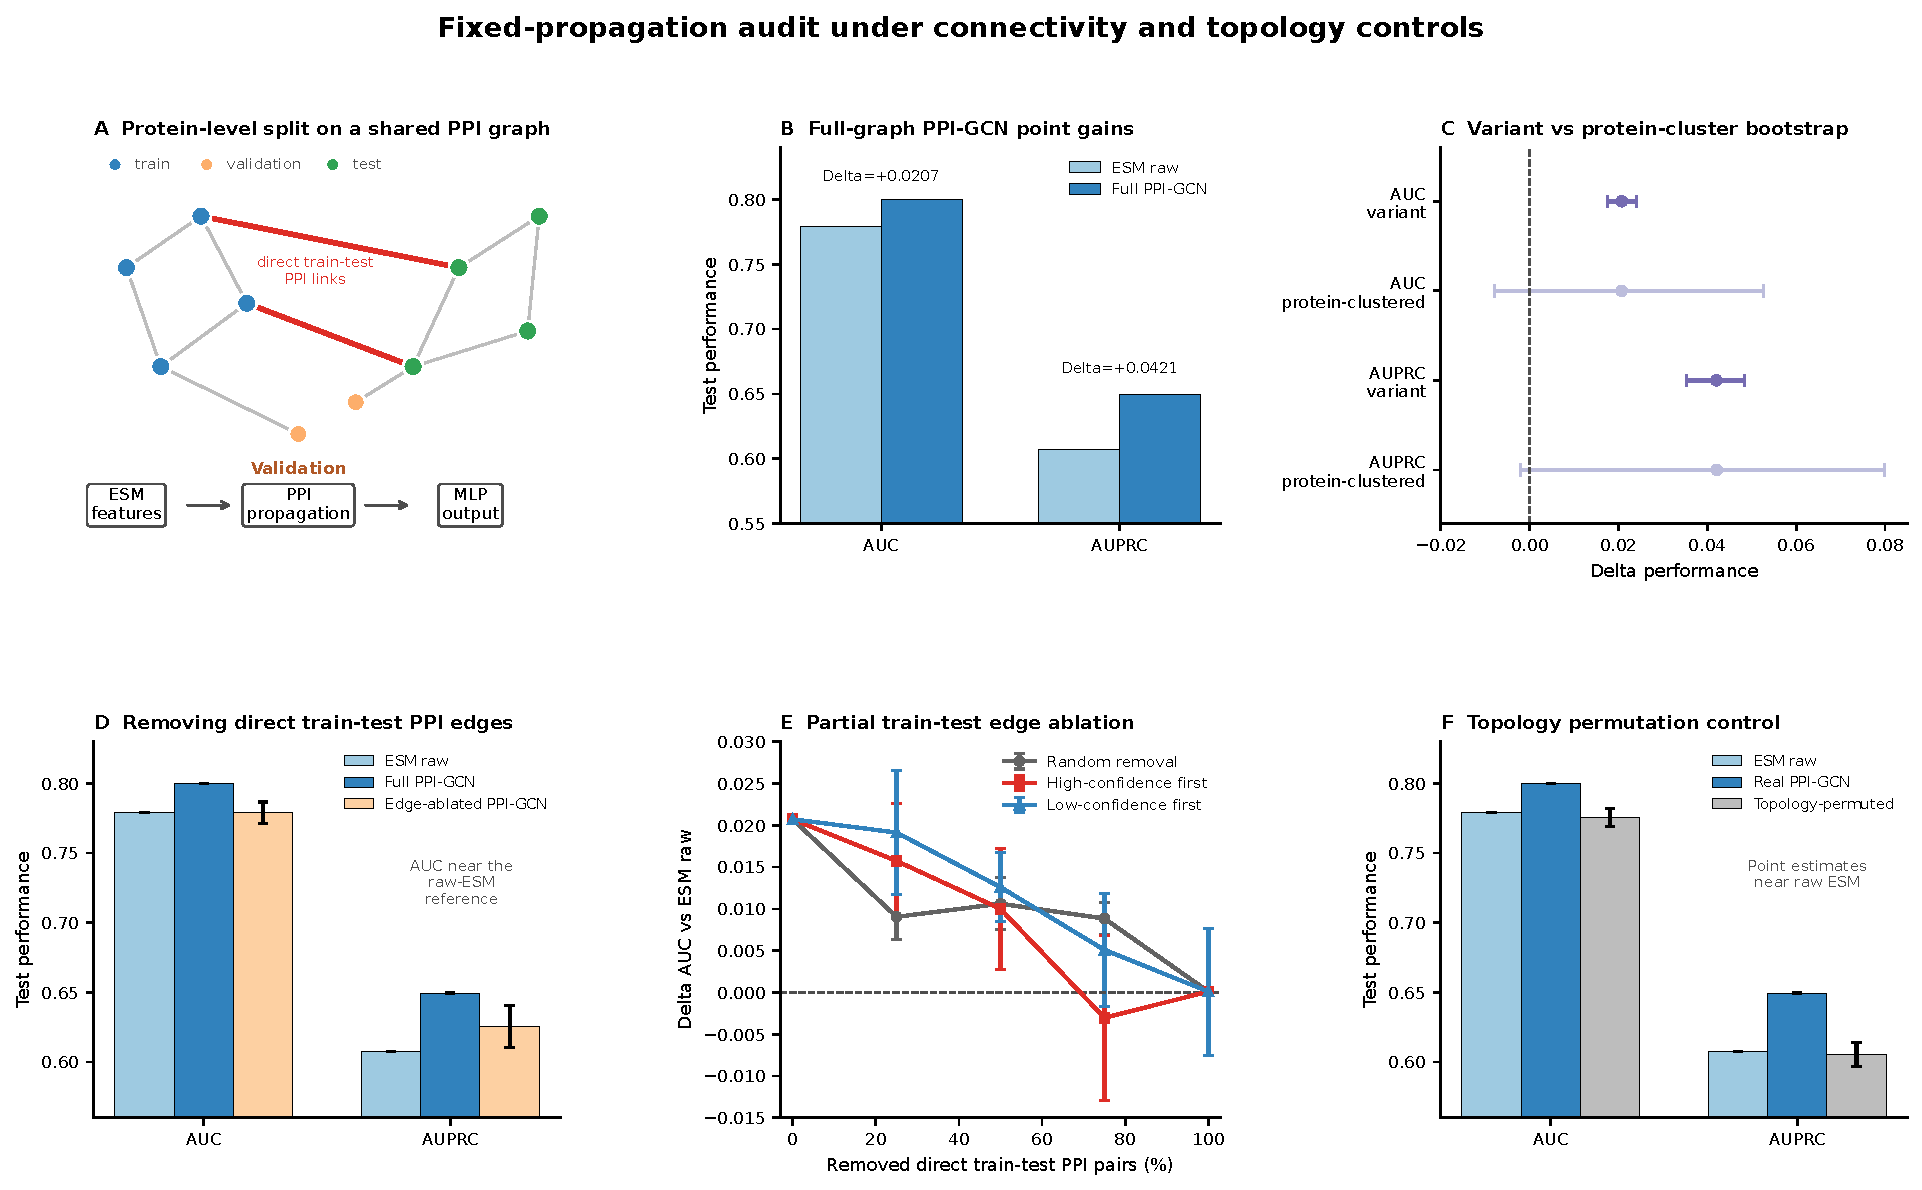
\includegraphics[width=0.98\textwidth]{figure_drafts/Figure1_connectivity_topology_controls_v2_accepted_minimal_clarified.pdf}
\caption{Workflow and historical audit of fixed PPI propagation. A, ESM features are propagated over STRING before downstream MLP classification; connectivity and topology controls probe the apparent gain. B/C, Retained reference pair and its variant/protein bootstrap intervals. Displayed differences follow the conventions in Supplementary Table 4A. D, Five historical edge-ablation fits compared with reference raw/full estimates. E, Historical partial-ablation curve; seeds, budgets and control operator are unmatched, and endpoints reused. F, Three graph permutations by three classifier seeds. Historical negative controls allow 30 epochs; the reference pair allows 50. Current common-protocol results are reported in the text and Supplementary Table 11.}
\label{fig:connectivity}
\end{figure*}

\subsection{Strong predictors and homology-aware evaluation bound PPI context gains}

Under the original split, single-score CADD and AlphaMissense baselines achieved AUC 0.9207 and 0.9470. In the historical fusion audit, the same-hidden-layer \CADDAM{} baseline reached mean AUC 0.9572; adding raw ESM, real PPI-GCN, edge-ablated or permuted representations gave 0.9680, 0.9718, 0.9708 and 0.9694 (Fig. 2B). The historical real-minus-raw fusion interval was positive, while ablated/permuted contrasts included zero (Fig. 2C). Current matched fusion yielded a small real-minus-raw margin ($\Delta$AUC +0.0032, protein 95\% CI [+0.0008, +0.0062]); the ablated contrast remained uncertain. The permutation contrast was small and positive conditional on the sampled graphs (Supplementary Table 12).

Under the homology-aware split, historical single-fit PPI-GCN exceeded raw ESM (AUC 0.7606 versus 0.7248; Fig. 2D). The retained graph-fusion estimate (0.9741) was lower than the repeated \CADDAM{} baseline (0.9754); raw fusion averaged 0.9728 (Fig. 2E). Current three-seed means were 0.9755 for scores, 0.9727 for raw fusion and 0.9752 for graph fusion. On ensemble predictions, graph-minus-score $\Delta$AUC was +0.0001, CI [-0.0019, +0.0020], and its AUPRC interval also crossed zero. The graph-versus-score effect remained uncertain under homology-aware splitting. Mean metrics and metrics of averaged probabilities can give different close rankings.

\begin{figure*}[!p]
\centering
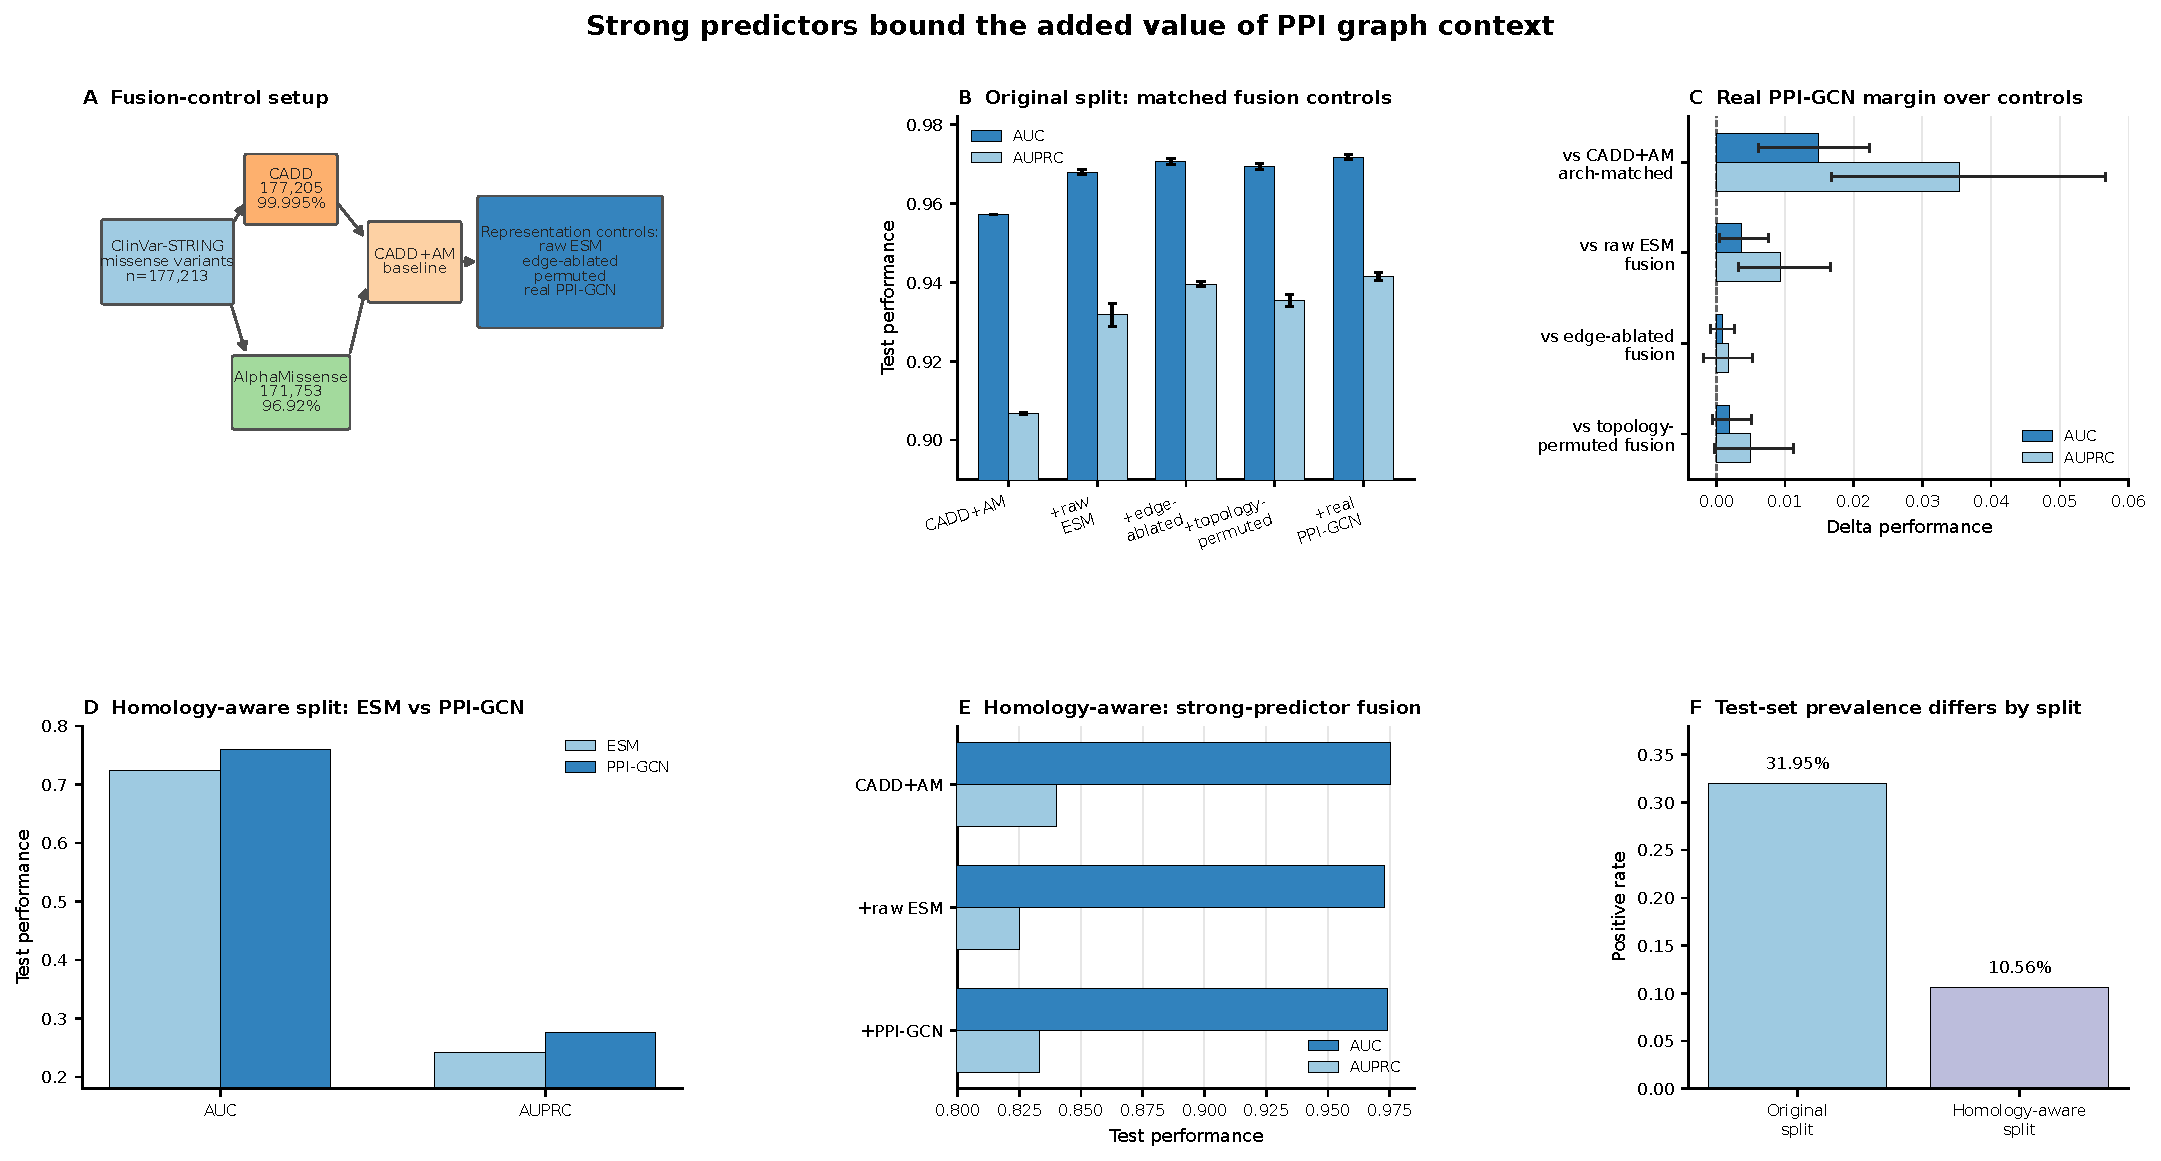
\includegraphics[width=0.98\textwidth]{figure_drafts/Figure2_fusion_homology_v1_accepted.pdf}
\caption{Historical fusion and homology-aware evaluation. A, Score coverage and fusion setup. Architecture-matched refers to the same hidden-layer architecture, not equal input-layer parameter counts or shared fitted weights. B, Original-split means and population SD across three classifier seeds per arm, except permuted fusion (3 graphs $\times$ 3 seeds). C, Ensemble differences with paired protein-bootstrap intervals, conditional on fitted models and sampled graphs. D, One retained representation fit per arm under homology splitting. E, Baseline/raw-fusion means use three fits; graph fusion uses one retained fit. F, Split prevalence. Current matched comparisons appear in the text and Supplementary Tables 11--12.}
\label{fig:fusion_homology}
\end{figure*}

\subsection{Exploratory graph gains across topology contexts}

ESM representation space showed modest correspondence with PPI topology. Neighbour pairs had mean cosine similarity 0.8789 versus 0.8639 for random pairs; within-community similarity also exceeded between-community similarity (Fig. 3A). Graph-associated gains were non-monotonic: mid-k-core variants showed $\Delta$AUC +0.0775, whereas high-degree variants showed -0.0178. Betweenness, clustering and neighbour-risk profiles varied across strata (Fig. 3B--D).

Exploratory joint maps included both positive and negative profiles, such as mid-k-core/high-betweenness ($\Delta$AUC +0.1429) and high-k-core/low-clustering (-0.0532; Fig. 3E/F). All 53 joint cells and highlighted profiles were inspected on the same test set. Their variant-resampled intervals do not account for protein dependence or post-hoc selection. These observations identify hypotheses for independent validation rather than confirmed benefiting subgroups.



\begin{figure*}[!p]
\centering
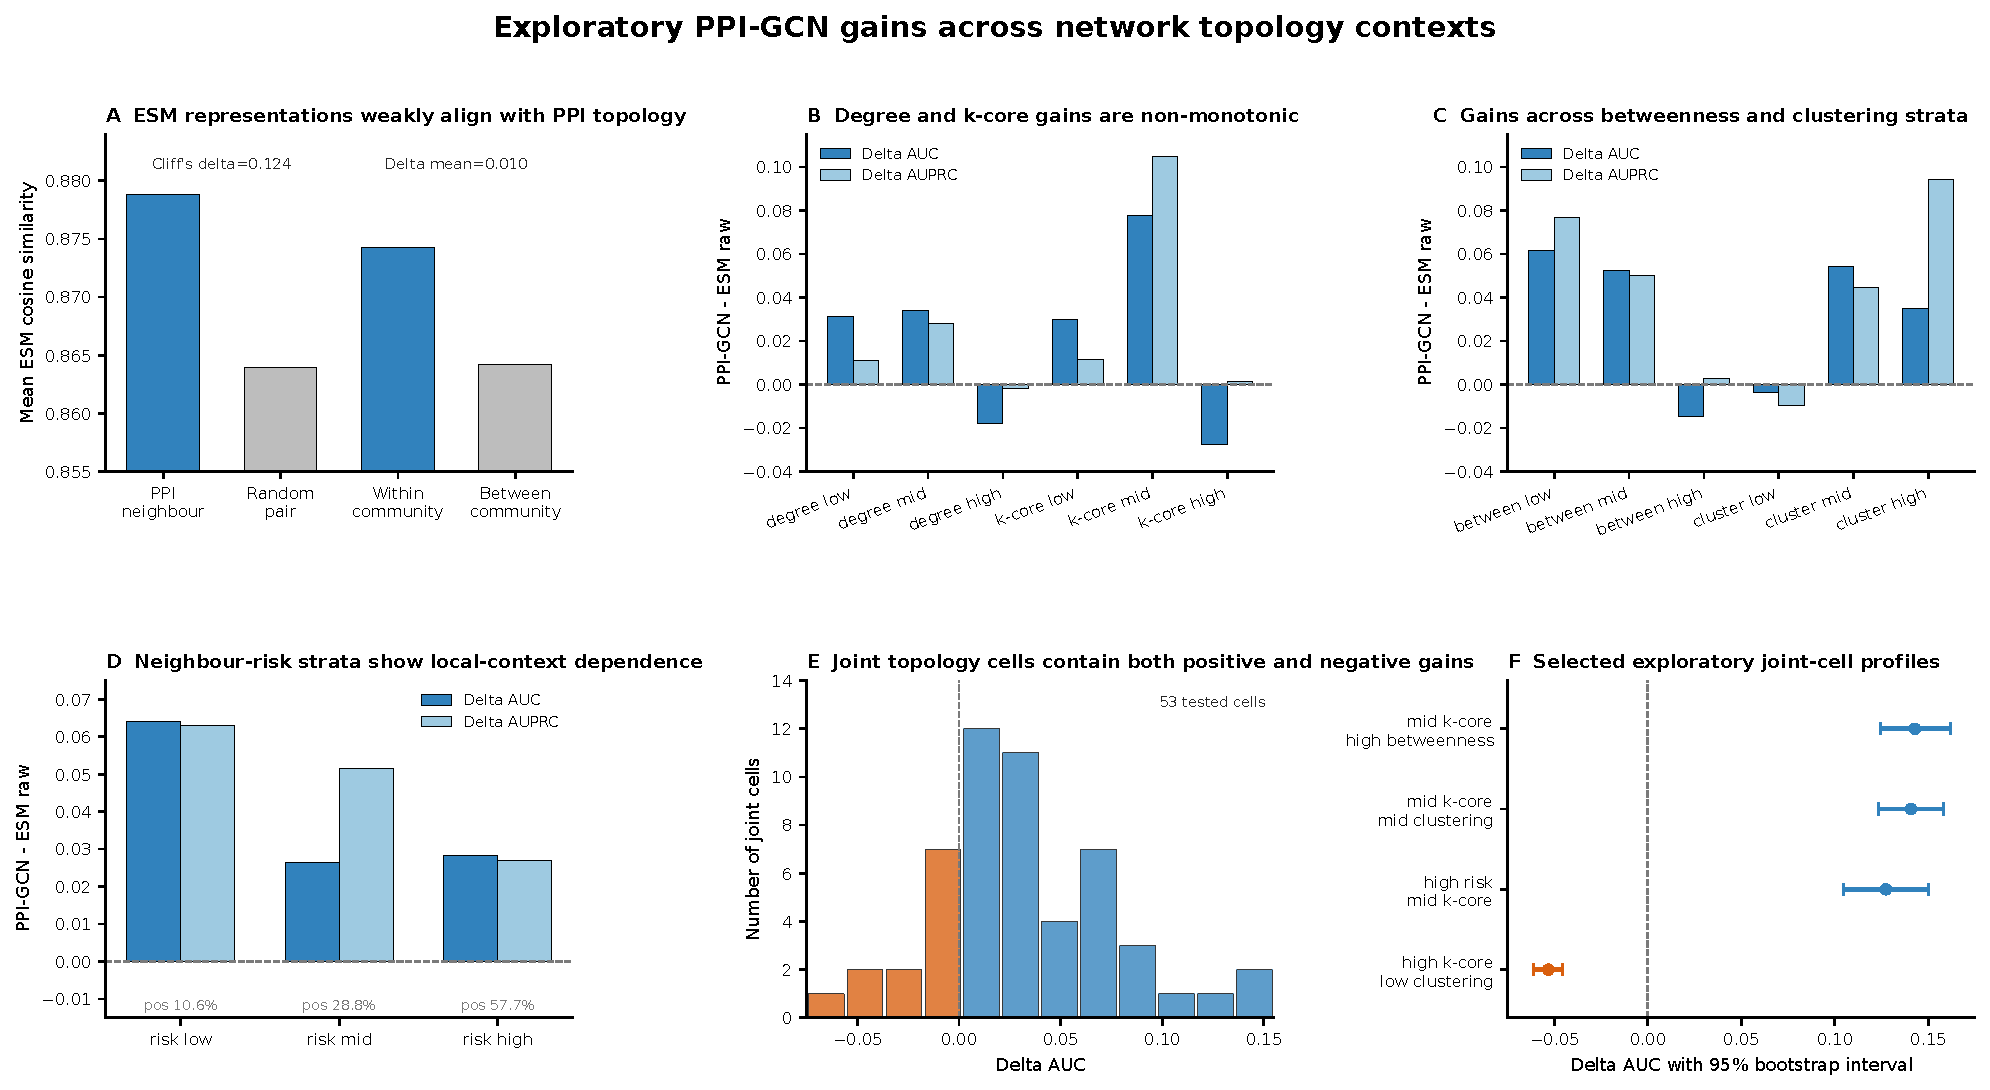
\includegraphics[width=0.98\textwidth]{figure_drafts/Figure3_topology_context_v1_accepted_clarified.pdf}
\caption{Exploratory topology-context profiles from retained reference predictions. A, ESM similarity by network relation. B--D, Gains across degree, k-core, betweenness, clustering and neighbour-risk strata. E/F, Joint-cell profiles selected from 53 inspected cells. These descriptive, post-hoc profiles are not independently confirmed; historical within-cell intervals omit protein dependence and selection uncertainty.}
\label{fig:topology_context}
\end{figure*}

\subsection{Graph augmentation reshapes false-negative and false-positive predictions differently}

At a fixed decision-score threshold of 0.5, raw ESM and PPI-GCN were jointly correct for 11,875 test variants and jointly wrong for 3,965. Graph propagation corrected 1,436 and degraded 944 variants: 837 false negatives were rescued and 599 false positives suppressed, while 904 true negatives and 40 true positives were degraded (Fig. 4A).

The retained-reference \CADDAM{} and graph-fusion pair corrected 666 variants and degraded 275, with more suppressed false positives than rescued false negatives (444 versus 222; Fig. 4B). This pair differs from the repeated-run fusion comparison in Fig. 2. Counts are conditional on the selected fits and threshold.

For the raw-ESM-to-PPI-GCN pair, rescued false negatives had higher degree, neighbour-risk and betweenness, whereas suppressed false positives had higher clustering and within-community neighbour fraction (Fig. 4C). Profiles for the retained fusion pair are shown in Fig. 4D. Directional mean profiles and error-stratified effect sizes are retained descriptively (Fig. 4E/F). The latter groups were stratified by baseline error, not matched on continuous prediction difficulty. Significance encodings are omitted because the old feature-wise tests ignored within-protein dependence. These profiles do not establish a mechanism for the prediction changes.

\begin{figure*}[!p]
\centering
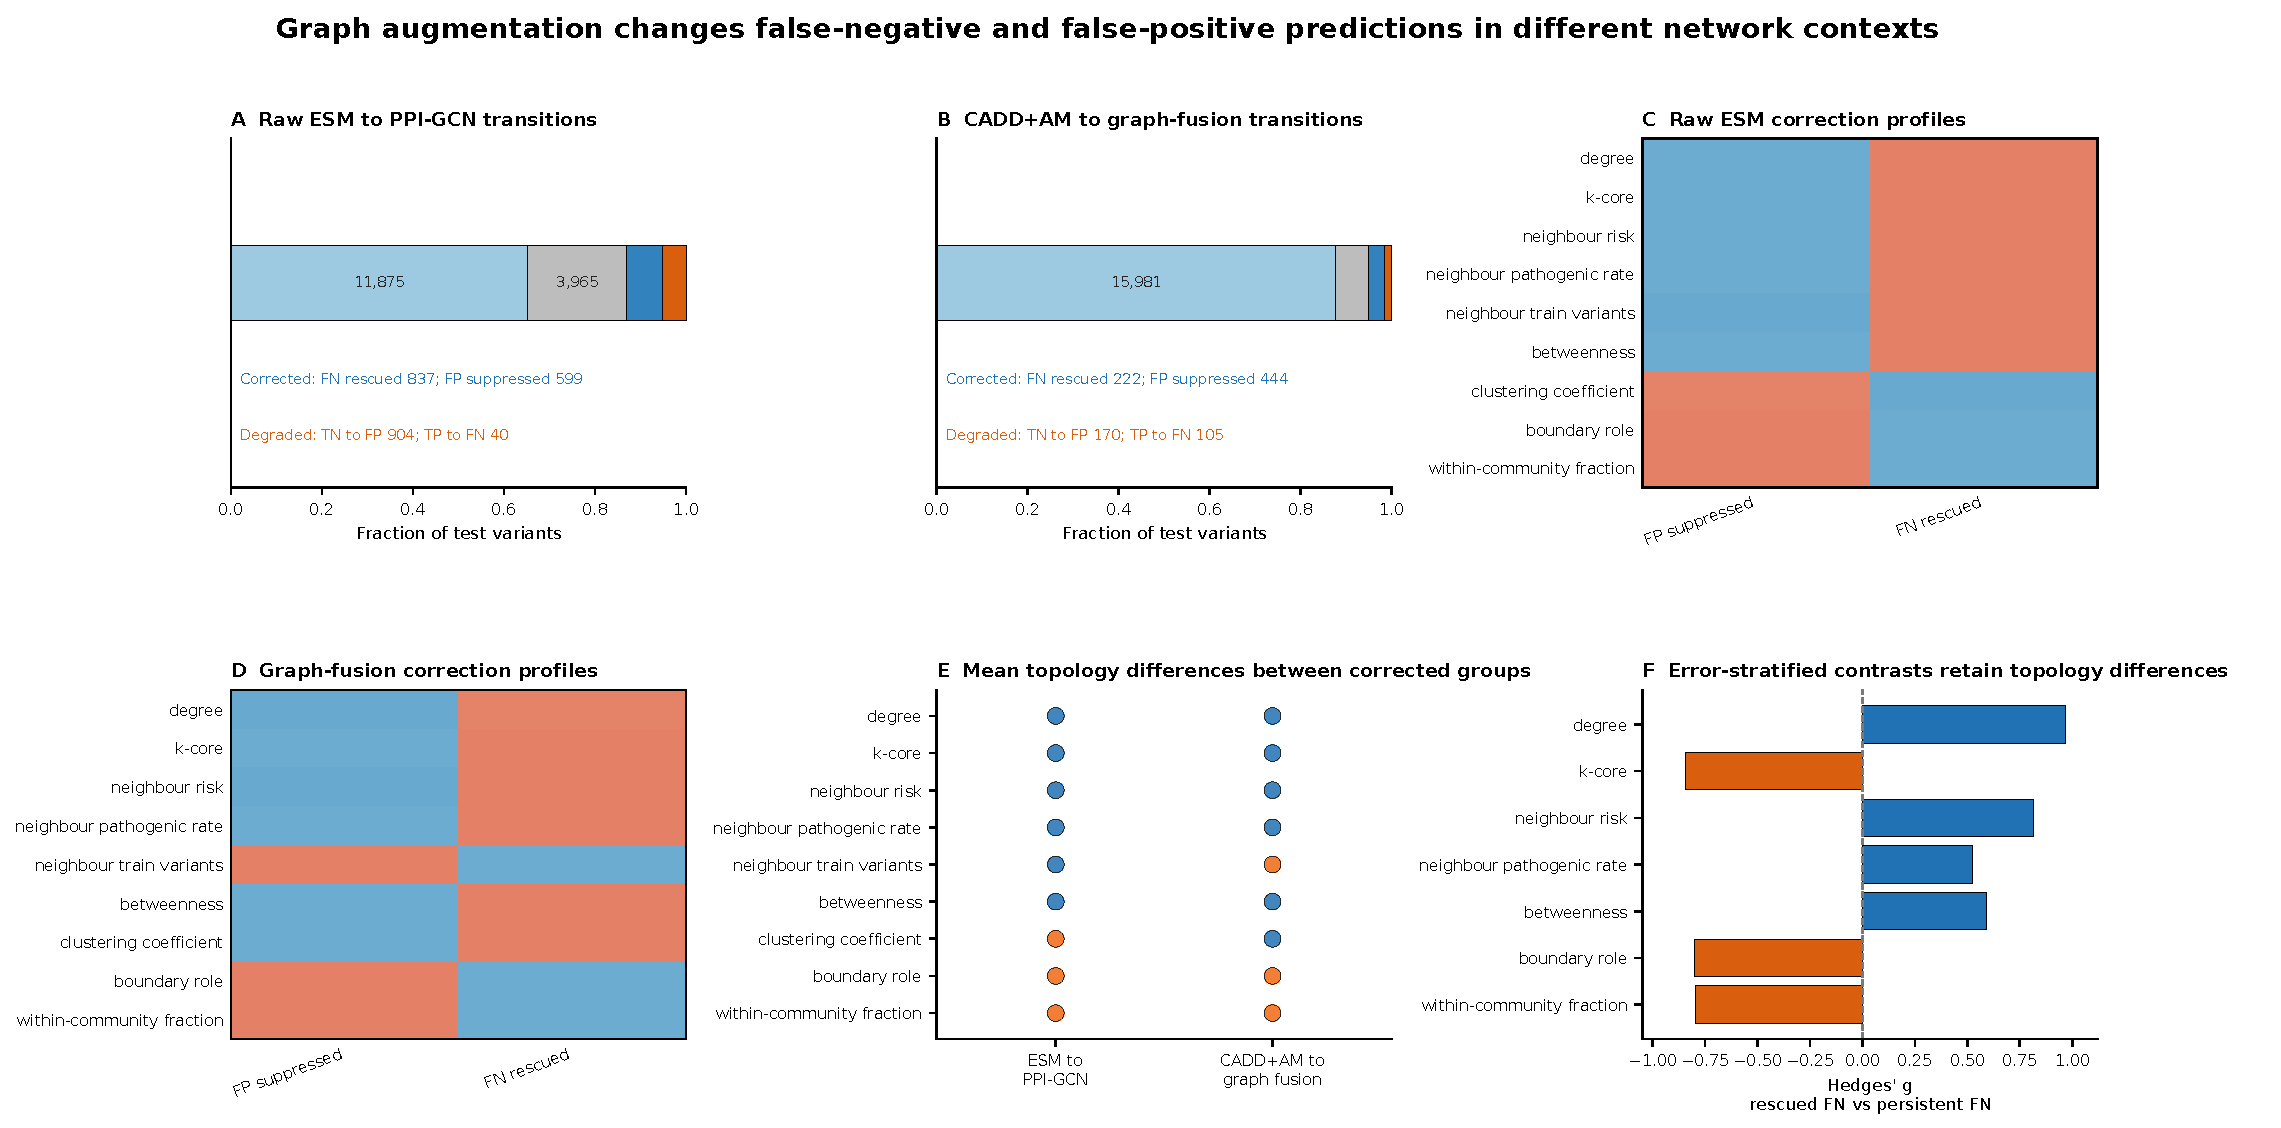
\includegraphics[width=0.98\textwidth]{figure_drafts/Figure4_prediction_transitions_v2_accepted_minimal_clarified.pdf}
\caption{Historical prediction transitions and descriptive topology profiles. A/B, Retained raw/graph and score/graph-fusion comparisons at threshold 0.5. C/D, Row-centered, range-scaled group means; warm/blue colors denote above/below the within-row mean, not comparable effect magnitudes across rows. E, Uniform blue/orange dots denote higher means among rescued false negatives/suppressed false positives, respectively. F, Baseline-error-stratified Hedges' \textit{g}; blue/orange denote positive/negative effects. Repeated variants within proteins limit inferential interpretation.}
\label{fig:prediction_transitions}
\end{figure*}


\subsection{External-source and second-network validation}

On the primary external set, mean AUC across three seeds was 0.6932 for raw ESM, 0.7304 for STRING propagation and 0.7025 for BioGRID. STRING-minus-raw ensemble gains were +0.0375 AUC (protein 95\% CI [+0.0173, +0.0564]) and +0.0463 AUPRC ([+0.0151, +0.0745]). The nested stricter subset supported the same AUC direction (+0.0352, [+0.0034, +0.0667]); BioGRID-versus-raw intervals crossed zero in both sets (Fig.~\ref{fig:external}A).

On the original split, BioGRID fusion improved over scores alone ($\Delta$AUC +0.0124, [+0.0034, +0.0210]), but its added benefit over raw-embedding fusion remained uncertain (+0.0009, [-0.0011, +0.0036]). BioGRID fusion was below STRING fusion under the fitted-ensemble intervals in both splits (Fig.~\ref{fig:external}B). External gains and fusion complementarity therefore depend on network choice and comparator.

\begin{figure*}[!p]
\centering
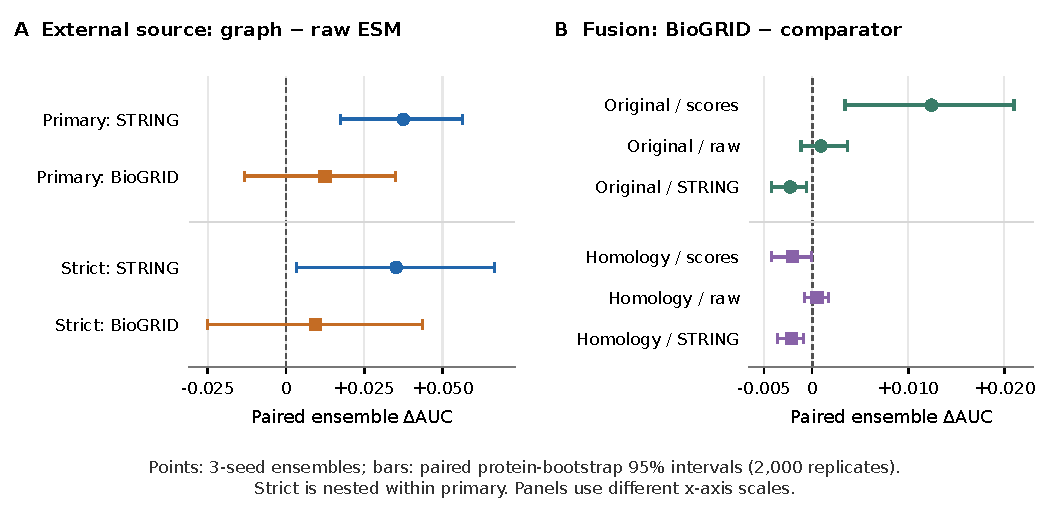
\includegraphics[width=0.98\textwidth]{figure_drafts/Figure5_external_validation.pdf}
\caption{Additional external-source and second-network validation. A, STRING/BioGRID propagation minus raw-ESM AUC on the primary HUMSAVAR set (10,785 variants; 2,498 proteins) and nested strict subset (6,934; 1,713). B, BioGRID fusion minus scores alone, raw-embedding fusion or STRING fusion in each split. Points use three-seed mean probabilities; bars are paired protein-bootstrap 95\% intervals (2,000 resamples), conditional on fitted models. Intervals are exploratory without multiplicity adjustment. All evaluated proteins remain frozen-graph nodes; the strict set is nested, not a second replication.}
\label{fig:external}
\end{figure*}

\section{Discussion}

PPI graph augmentation improved benchmark performance in the shared-graph evaluation, with effects that varied by evaluation design and baseline choice. The historical and matched audits show sensitivity to graph connectivity, but protein-level uncertainty limits the full-versus-raw claim. With \CADDAM{} included, protein-representation controls retained much of the gain, while the current real-minus-raw fusion margin was small and positive. These results support representation complementarity with a limited additional STRING margin under the original split.

Under the homology-aware split, the historical graph-fusion point was below the repeated score baseline, but the current matched graph-versus-score interval spanned zero. Additional input weights, redundant high-dimensional features, overfitting, feature scaling and changed protein composition are possible explanations for weaker fusion; these mechanisms were not experimentally separated. The prevalence shift limits cross-split AUPRC comparisons.

Graph propagation changed predictions in heterogeneous topology contexts. The observed profiles may reflect densely connected functional neighbourhoods or boundary-like network roles, but their post-hoc selection requires independent confirmation. External HUMSAVAR validation supports STRING transfer under the stated exclusions; BioGRID's uncertain incremental gains limit generalization across networks. Both databases may share underlying evidence, and the networks overlap. This is not independent-patient or prospective validation.

The evaluation has several constraints. ClinVar labels may reflect submission bias and future updates \cite{Landrum2020ClinVar}. Unknown development-data overlap for CADD and AlphaMissense limits prospective interpretation. Protein-level mapping omits isoform and residue-specific effects. STRING associations extend beyond direct physical interactions \cite{Szklarczyk2023STRING}; transductive propagation and direct-edge ablation retain indirect cross-partition paths. Outputs from class-weighted training are not calibrated clinical probabilities, and transition counts depend on the chosen threshold. The external set excludes specified variants/proteins but not all homologues or shared annotation evidence; external clinical-score fusion was not evaluated. These findings concern fixed propagation and should not be generalized to trained graph neural networks.

\noindent\textit{Practical recommendations:}
Compare graph features with raw embeddings and strong score baselines under matched training settings. State whether held-out proteins remain visible in the graph, assess uncertainty at the protein level, and treat selected topology groups as hypotheses. Check calibration and decision thresholds before clinical use.

\section*{Data and Code Availability}

Supplementary Information, code, compact source data, complete sample memberships, per-seed predictions, protocols and checksums are publicly available at \url{https://github.com/brynn-t02/ppi-graph-missense-audit}. Large provider resources, feature tensors and model checkpoints are stored separately; third-party source data should be obtained from their original providers.

\section*{Acknowledgment}

OpenAI ChatGPT, OpenAI Codex and Anthropic Claude assisted with literature organization, code development for the Methods and Results analyses, and manuscript language editing. AI-assisted scripts supported environment restoration, model fitting, data checks and statistical analysis. The authors take responsibility for reviewing the code, outputs, interpretation, references and final manuscript.

\IEEEtriggeratref{26}
\begin{thebibliography}{99}
\bibitem{Kircher2014CADD} M. Kircher et al., ``A general framework for estimating the relative pathogenicity of human genetic variants,'' \emph{Nature Genetics}, vol. 46, pp. 310--315, 2014, doi: 10.1038/ng.2892.
\bibitem{Ioannidis2016REVEL} N. M. Ioannidis et al., ``REVEL: an ensemble method for predicting the pathogenicity of rare missense variants,'' \emph{American Journal of Human Genetics}, vol. 99, pp. 877--885, 2016, doi: 10.1016/j.ajhg.2016.08.016.
\bibitem{Qi2021MVP} H. Qi et al., ``MVP predicts the pathogenicity of missense variants by deep learning,'' \emph{Nature Communications}, vol. 12, p. 510, 2021, doi: 10.1038/s41467-020-20847-0.
\bibitem{Sundaram2018PrimateAI} L. Sundaram et al., ``Predicting the clinical impact of human mutation with deep neural networks,'' \emph{Nature Genetics}, vol. 50, pp. 1161--1170, 2018, doi: 10.1038/s41588-018-0167-z.
\bibitem{Frazer2021EVE} J. Frazer et al., ``Disease variant prediction with deep generative models of evolutionary data,'' \emph{Nature}, vol. 599, pp. 91--95, 2021, doi: 10.1038/s41586-021-04043-8.
\bibitem{Cheng2023AlphaMissense} J. Cheng et al., ``Accurate proteome-wide missense variant effect prediction with AlphaMissense,'' \emph{Science}, vol. 381, eadg7492, 2023, doi: 10.1126/science.adg7492.
\bibitem{Lin2023ESM} Z. Lin et al., ``Evolutionary-scale prediction of atomic-level protein structure with a language model,'' \emph{Science}, vol. 379, pp. 1123--1130, 2023, doi: 10.1126/science.ade2574.
\bibitem{Barabasi2011NetworkMedicine} A.-L. Barabasi, N. Gulbahce, and J. Loscalzo, ``Network medicine: a network-based approach to human disease,'' \emph{Nature Reviews Genetics}, vol. 12, pp. 56--68, 2011, doi: 10.1038/nrg2918.
\bibitem{Menche2015DiseaseModules} J. Menche et al., ``Disease networks. Uncovering disease-disease relationships through the incomplete interactome,'' \emph{Science}, vol. 347, 1257601, 2015, doi: 10.1126/science.1257601.
\bibitem{Sahni2015InteractionPerturbation} N. Sahni et al., ``Widespread macromolecular interaction perturbations in human genetic disorders,'' \emph{Cell}, vol. 161, pp. 647--660, 2015, doi: 10.1016/j.cell.2015.04.013.
\bibitem{Chen2018InteractomePerturbation} S. Chen et al., ``An interactome perturbation framework prioritizes damaging missense mutations for developmental disorders,'' \emph{Nature Genetics}, vol. 50, pp. 1032--1040, 2018, doi: 10.1038/s41588-018-0130-z.
\bibitem{Yates2014SuSPect} C. M. Yates, I. Filippis, L. A. Kelley, and M. J. E. Sternberg, ``SuSPect: enhanced prediction of single amino acid variant (SAV) phenotype using network features,'' \emph{Journal of Molecular Biology}, vol. 426, pp. 2692--2701, 2014, doi: 10.1016/j.jmb.2014.04.026.
\bibitem{Ozturk2022NetworkFeatures} K. Ozturk and H. Carter, ``Predicting functional consequences of mutations using molecular interaction network features,'' \emph{Human Genetics}, vol. 141, pp. 1195--1210, 2022, doi: 10.1007/s00439-021-02329-5.
\bibitem{Zhang2022gMVP} H. Zhang, M. S. Xu, X. Fan, W. K. Chung, and Y. Shen, ``Predicting functional effect of missense variants using graph attention neural networks,'' \emph{Nature Machine Intelligence}, vol. 4, no. 11, pp. 1017--1028, 2022, doi: 10.1038/s42256-022-00561-w.
\bibitem{Cheng2021VEGN} J. Cheng, C. Lawrence, and M. Niepert, ``VEGN: variant effect prediction with graph neural networks,'' arXiv:2106.13642, 2021, doi: 10.48550/arXiv.2106.13642.
\bibitem{Yu2025GNNMAP} H. Yu et al., ``A graph neural network approach for accurate prediction of pathogenicity in multi-type variants,'' \emph{Briefings in Bioinformatics}, vol. 26, bbaf151, 2025, doi: 10.1093/bib/bbaf151.
\bibitem{Ghadie2025DiseaseSpecificGNN} M. Ghadie, S. Sardaar, and Y. Trakadis, ``Disease-specific prediction of missense variant pathogenicity with DNA language models and graph neural networks,'' \emph{Bioengineering}, vol. 12, p. 1098, 2025, doi: 10.3390/bioengineering12101098.
\bibitem{Littmann2022ProteinMLTips} Q. Hou, K. Waury, D. Gogishvili, and K. A. Feenstra, ``Ten quick tips for sequence-based prediction of protein properties using machine learning,'' \emph{PLOS Computational Biology}, vol. 18, no. 12, Art. no. e1010669, 2022, doi: 10.1371/journal.pcbi.1010669.
\bibitem{Teufel2023GraphPart} F. Teufel, M. H. Gislason, J. J. Almagro Armenteros, A. R. Johansen, O. Winther, and H. Nielsen, ``GraphPart: homology partitioning for biological sequence analysis,'' \emph{NAR Genomics and Bioinformatics}, vol. 5, lqad088, 2023, doi: 10.1093/nargab/lqad088.
\bibitem{Landrum2020ClinVar} M. J. Landrum et al., ``ClinVar: improvements to accessing data,'' \emph{Nucleic Acids Research}, vol. 48, pp. D835--D844, 2020, doi: 10.1093/nar/gkz972.
\bibitem{Szklarczyk2023STRING} D. Szklarczyk et al., ``The STRING database in 2023: protein-protein association networks and functional enrichment analyses for any sequenced genome of interest,'' \emph{Nucleic Acids Research}, vol. 51, pp. D638--D646, 2023, doi: 10.1093/nar/gkac1000.
\bibitem{Kipf2017GCN} T. N. Kipf and M. Welling, ``Semi-supervised classification with graph convolutional networks,'' \emph{International Conference on Learning Representations}, 2017.
\bibitem{Steinegger2017MMseqs2} M. Steinegger and J. Soding, ``MMseqs2 enables sensitive protein sequence searching for the analysis of massive data sets,'' \emph{Nature Biotechnology}, vol. 35, pp. 1026--1028, 2017, doi: 10.1038/nbt.3988.
\bibitem{Kingma2015Adam} D. P. Kingma and J. Ba, ``Adam: a method for stochastic optimization,'' \emph{International Conference on Learning Representations}, 2015, arXiv:1412.6980.
\bibitem{Schubach2024CADDv17} M. Schubach et al., ``CADD v1.7: using protein language models, regulatory CNNs and other nucleotide-level scores to improve genome-wide variant predictions,'' \emph{Nucleic Acids Research}, vol. 52, no. D1, pp. D1143--D1154, 2024, doi: 10.1093/nar/gkad989.
\bibitem{Efron1993Bootstrap} B. Efron and R. J. Tibshirani, \emph{An Introduction to the Bootstrap}. Chapman \& Hall/CRC, 1993.
\bibitem{Benjamini1995FDR} Y. Benjamini and Y. Hochberg, ``Controlling the false discovery rate: a practical and powerful approach to multiple testing,'' \emph{Journal of the Royal Statistical Society: Series B}, vol. 57, pp. 289--300, 1995, doi: 10.1111/j.2517-6161.1995.tb02031.x.
\bibitem{Saito2015PrecisionRecall} T. Saito and M. Rehmsmeier, ``The precision-recall plot is more informative than the ROC plot when evaluating binary classifiers on imbalanced datasets,'' \emph{PLOS ONE}, vol. 10, e0118432, 2015, doi: 10.1371/journal.pone.0118432.
\bibitem{UniProt2025} The UniProt Consortium, ``UniProt: the Universal Protein Knowledgebase in 2025,'' \emph{Nucleic Acids Research}, vol. 53, no. D1, pp. D609--D617, 2025, doi: 10.1093/nar/gkae1010.
\bibitem{Stark2006BioGRID} C. Stark, B.-J. Breitkreutz, T. Reguly, L. Boucher, A. Breitkreutz, and M. Tyers, ``BioGRID: a general repository for interaction datasets,'' \emph{Nucleic Acids Research}, vol. 34, pp. D535--D539, 2006, doi: 10.1093/nar/gkj109.
\end{thebibliography}
\end{document}
